\documentclass{beamer}

\usepackage[utf8]{inputenc}
% Replace caption colon with period (e.g. "Figure 1: ..." -> "Figure 1. ..."):
\usepackage[labelsep=period]{caption}

\usetheme{Madrid}
\usecolortheme{default}

%************************************** DOC LINKS ************************************************
%** Beamer         - https://www.overleaf.com/learn/latex/Beamer                                **
%** TOC            - https://www.overleaf.com/learn/latex/Table_of_contents                     **
%** Colors         - https://www.overleaf.com/learn/latex/Using_colours_in_LaTeX                **
%** Fonts          - https://www.overleaf.com/learn/latex/Font_sizes,_families,_and_styles      **
%** Madrid theme   - https://www.overleaf.com/project/5ceee72c18cd5947169c7404                  **
%** Beamer styling - http://www.cpt.univ-mrs.fr/~masson/latex/Beamer-appearance-cheat-sheet.pdf **
%** Commands       - https://www.overleaf.com/learn/latex/Commands                              **
%** Environments   - https://www.overleaf.com/learn/latex/Environments                          **
%** Beamer source  - https://github.com/josephwright/beamer                                     **
%** Counters       - https://www.overleaf.com/learn/latex/Counters                              **
%** Hyperlinks     - https://www.overleaf.com/learn/latex/Hyperlinks                            **
%*************************************************************************************************

% BEG COLOR SCHEME
%-----------------
% BEG CUSTOM COLORS
% Color values retrieved from slide templates uploaded to https://www.ttu.ee/ulikool/tutvustus/logo/
\definecolor{TalTechPurple}{rgb}{0.67, 0.07, 0.32}     % RGB(171, 19, 18)   / 255
\definecolor{TalTechPink}{rgb}{0.89, 0.02, 0.49}       % RGB(228, 6, 126)   / 255
\definecolor{TalTechGray}{rgb}{0.58, 0.59, 0.69}       % RGB(147, 150, 176) / 255
\definecolor{TalTechDarkPurple}{rgb}{0.20, 0.17, 0.27} % RGB(51, 43, 69)    / 255
\definecolor{LightGray}{rgb}{0.95, 0.95, 0.95}         % RGB(242, 242, 242) / 255
% END CUSTOM COLORS

% BEG FRAME COLORS
\setbeamercolor{title}{bg=TalTechPurple}
\setbeamercolor{frametitle}{bg=TalTechPurple}
% END FRAME COLORS

% BEG HEADER/FOOTER COLORS
\setbeamercolor{author in head/foot}{bg=TalTechPurple}
\setbeamercolor{title in head/foot}{bg=TalTechGray}
\setbeamercolor{date in head/foot}{bg=TalTechPurple}
% END HEADER/FOOTER COLORS

% BEG TOC COLORS
\setbeamercolor{section in toc}{fg=black}
\setbeamercolor{section number projected}{bg=TalTechPink}
% END TOC COLORS

% BEG ELEMENT COLORS
% Item lists:
\setbeamercolor{item projected}{bg=TalTechPink}
\setbeamercolor{subitem projected}{bg=TalTechPink}
\setbeamercolor{subsubitem projected}{bg=TalTechPink}

% Blocks:
\setbeamercolor{block title}{bg=TalTechPurple}
\setbeamercolor{block body}{bg=LightGray}
\setbeamercolor{postit}{fg=black, bg=LightGray}

% Captions:
\setbeamercolor{caption name}{fg=TalTechPurple}
\setbeamerfont{caption}{series=\normalfont,size=\fontsize{7}{8}}
% END ELEMENT COLORS
%-----------------
% END COLOR SCHEME

% BEG CONFIGURATION
%------------------
% BEG FOOTLINE
\newcommand{\configurefootline}[1]{
    \setbeamertemplate{footline}{
      \leavevmode
      \hbox{% Default: wd=.333333
            \begin{beamercolorbox}[wd=.3\paperwidth,ht=2.8ex,dp=1ex,center]{author in head/foot}%
                \usebeamerfont{author in head/foot}
                \insertshortauthor\ (\insertshortinstitute)
            \end{beamercolorbox}%
    
            \begin{beamercolorbox}[wd=.4\paperwidth,ht=2.8ex,dp=1ex,center]{title in head/foot}%
                \usebeamerfont{title in head/foot}
                \insertshorttitle
            \end{beamercolorbox}%
    
            \begin{beamercolorbox}[wd=.3\paperwidth,ht=2.8ex,dp=1ex,center]{date in head/foot}%
                \usebeamerfont{date in head/foot}
                \insertshortdate{}%
                \ifnum1=#1 % Not pretty.
                    \hspace*{1em}%
                    \insertframenumber{} / 
                    \inserttotalframenumber%
                    \hspace*{2ex}%
                %\else
                %    \hspace*{3em}
                \fi
            \end{beamercolorbox}%
        }
        \vskip0pt%
    }
}
% END FOOTLINE

% BEG NAVIGATION CONTROLS
%========================
% BEG FRAME NAV CONTROL DEFINITION:
%==================================
\makeatletter
\newcounter{prevframecntr}

\newcommand{\inserttargetforprevframe}[1]{%
    \setcounter{prevframecntr}{#1}%
    \addtocounter{prevframecntr}{-1}%
    \hypertarget{NextFrameEnd\theprevframecntr}%
}
\newcommand{\insertnextframeendlink}[1]{%
    \hyperlink{NextFrameEnd#1}%
}

% Variables (from Beamer src - https://github.com/josephwright/beamer):
\def\beamer@framepages#1#2{%
% Call: \beamer@framepages{\beamer@framestartpage}{\beamer@frameendpage}}
    \ifnum\c@page<#1%       Cond: page < frame start page           (before frame)
    \else%
        \ifnum\c@page>#2%   Cond: page > frame end                  (after frame)
        \else%              Cond: frame start <= page <= frame end  (within frame)
            \ifnum\c@page=#2% Bit of a hack here:
                % Note: will loop back to start because the final hyperlink is not defined.
                \inserttargetforprevframe{\theframenumber}\relax%
            \fi%
            \gdef\beamer@startpageofframe{#1}\relax%
            \gdef\beamer@endpageofframe{#2}\relax%
        \fi%
    \fi%
}

\def\beamer@nextpage#1{%
    \beamer@tempcount=#1%
    \advance\beamer@tempcount by1\relax%
    \ifnum\beamer@tempcount>\beamer@endpageofdocument%
        \beamer@tempcount=\beamer@endpageofdocument%
    \fi
}
\def\beamer@prevpage#1{%
    \beamer@tempcount=#1\relax%
    \ifnum\beamer@tempcount>1%
        \advance\beamer@tempcount by-1%
    \fi%
}

% Hyperlinks (from Beamer src):
\def\hyperlinkframeendprev{%
    \beamer@prevpage\beamer@startpageofframe%
    \hyperlink{Navigation\the\beamer@tempcount}%
}
\def\hyperlinkframestart{%
    \hyperlink{Navigation\beamer@startpageofframe}%
}
\def\hyperlinkframeend{%
    \hyperlink{Navigation\beamer@endpageofframe}%
}
\def\hyperlinkframestartnext{%
% Sets(!) beamer page counter (\beamer@tempcount) to @endpageofframe (last page of current frame), and increments counter.
%  @startpageofframe, @endpageofframe are set on entry to frame (\def\beamer@writeslidentry...).
% \beamer@endpageofframe is handed as arg
    \beamer@nextpage\beamer@endpageofframe%
    \hyperlink{Navigation\the\beamer@tempcount}%
}
% Customized hyperlinkframestartnext:
\def\hyperlinkframeendnext{
    \beamer@nextpage\beamer@endpageofframe%
    \insertnextframeendlink{\theframenumber}
}

% Symbols (from Beamer src):
\def\insertframenavigationsymbol{%
    % Background icon:
    \begin{pgfpicture}{0pt}{-1.5pt}{20pt}{5.5pt}
        \pgfuseobject{beamerframenavstrong}%
        \usebeamercolor[fg]{navigation symbols dimmed}
        \pgfuseobject{beamerframenavlight}%
    \end{pgfpicture}\kern-20pt%
    % Hyperlinks:
    \hyperlinkframeendprev{\beamer@linkspace{5pt}}%     - Left triangle (nav to end of prev).
    \hyperlinkframestart{\beamer@linkspace{5pt}}%       - Left triangle (inside frame).
    \hyperlinkframeend{\beamer@linkspace{5pt}}%         - Middle square (nav to end of current).
    %\hyperlinkframestartnext{\beamer@linkspace{5pt}}%  - Right triangle (nav to beg next).
    % Override:
    \hyperlinkframeendnext{\beamer@linkspace{5pt}}%
}
\makeatother
%==================================
% END FRAME NAV CONTROL DEFINITION:

\setbeamertemplate{navigation symbols}{
    \hbox{\insertslidenavigationsymbol}
    \hbox{\insertframenavigationsymbol}
%    \hbox{\insertsectionnavigationsymbol}
%    \hbox{\insertsubsectionnavigationsymbol}
%    \hbox{\insertdocnavigationsymbol}
    \hbox{\insertbackfindforwardnavigationsymbol}
}
%========================
% END NAVIGATION CONTROLS

% Add numbering to captions:
\setbeamertemplate{caption}[numbered]

%------------------
% END CONFIGURATION

% UTILITIES
%----------
% Global \renewcommand:
\makeatletter
\def\gnewcommand{\g@star@or@long\new@command}
\def\grenewcommand{\g@star@or@long\renew@command}
\def\g@star@or@long#1{% 
      \@ifstar{\let\l@ngrel@x\global#1}{\def\l@ngrel@x{\long\global}#1}}
\makeatother
% from (https://tex.stackexchange.com/questions/51733/global-renewcommand-equivalent-of-global-def)

\newcommand{\recallframetitle}{}
\newcommand{\storeframetitle}[1]{%
    \grenewcommand{\recallframetitle}{#1}%
}
\newcommand{\frametitlestore}[1]{
    \frametitle{#1}%
    \storeframetitle{#1}%
}
\newcommand{\frametitlestorepause}[1]{%
    \frametitlestore{#1}%
    \pause%
}
\newcommand{\frametitlestorecont}[1]{%
    \frametitle{#1 (cont'd)}%
    \storeframetitle{#1}%
}
\newcommand{\frametitlecont}{%
    \frametitle{\recallframetitle{} (cont'd)}%
}

\newcommand{\pauseafteritemize}{\pause[\thebeamerpauses]}
\newcommand{\monofont}[1]{{\footnotesize \texttt{#1}}}
% https://tex.stackexchange.com/questions/9363/how-does-one-insert-a-backslash-or-a-tilde-into-latex:
\newcommand{\vertmidtilde}[0]{{\raise.17ex\hbox{$\scriptstyle\sim$}}}
\newenvironment{textbox}
    {\begin{beamercolorbox}[wd=\textwidth,rounded=true,shadow=true]{postit}}
    {\end{beamercolorbox}}
\newenvironment{definitionbox}[1][]
    {\begin{block}{#1} \pause}
    {\end{block}}
\newenvironment{definitionboxnopause}[1][]
    {\begin{block}{#1}}
    {\end{block}}

\newcommand{\TDLTP}{\texorpdfstring{TDL\textsuperscript{TP}}{TDL(TP)}}
%----------
% UTILITIES

% BEG TITLE PAGE/SHARED DATA
\title[Implementation of an Interpreter for \TDLTP{}]{
    Implementation of an Interpreter for
    the Test Purpose Specification Language \TDLTP{}
}
\author[Tanel Prikk]{
    Tanel Prikk
    \texorpdfstring{\\[1.5ex]}{, }
    \small{Supervisor: Jüri Vain, PhD}
    \texorpdfstring{\\[0.5ex]}{, }
    \small{Co-supervisor: Evelin Halling, PhD}
}
\institute[TalTech]{
    Tallinn University of Technology\\[1ex]
    School of Information Technologies
}
\date[June 12, 2019]{2019}
% Should skip the logo. Implies TalTech created the slide templates, but this isn't the case.
%\logo{
%    \raisebox{-0.2cm}[0pt][0pt]{%
%        % Icon retrieved from https://www.ttu.ee/ulikool/tutvustus/logo/
%        \includegraphics[height=0.75cm]{images/theme/TalTechLogo.png}
%    }%
%}
% END TITLE PAGE/SHARED DATA

% BEG SECTION OUTLINE
\AtBeginSection[]{
    \begingroup
        % Remove slide count from footline:
        \configurefootline{0}

        \begin{frame}[noframenumbering] % Shrink to fit: shrink=1.5
            \frametitle{Next Section}
            \tableofcontents[
                currentsection,
                currentsubsection,
                % Only expand current section:
                subsectionstyle=show/show/hide
            ]
        \end{frame}
    \endgroup
}
% END SECTION OUTLINE

\begin{document}
    \configurefootline{1} % Init footline.
% BEG TITLE FRAME
    \begingroup
        % Remove footer:
        \setbeamertemplate{footline}{}
        % Remove logo:
        \setbeamertemplate{logo}{}
        % Remove nav controls (bottom right):
        \setbeamertemplate{navigation symbols}{}

        \frame[noframenumbering]{
            \titlepage
        }
    \endgroup
% END TITLE FRAME

% BEG CONTENT FRAMES
%===================
    \begin{frame} % Outline frame.
        \frametitle{Presentation Outline}
        % Show top level sections only:
        \tableofcontents[subsectionstyle=show/hide/hide]
    \end{frame}

% BEG SECTION: CONTEXT
%---------------------
    \section{Context}
% BEG SUBSECTION: MBT
    \subsection{Model-Based Testing}
    \begin{frame}
        \frametitlestore{Context -- Model-Based Testing}
        \begin{definitionboxnopause}[Model-Based Testing (MBT)]
            Black-box testing method where explicit models derived from requirements are used to verify the correctness of a system under test (SUT).
        \end{definitionboxnopause}
        \pause
        \begin{figure}
            \includegraphics<1,2>[height=0.5\textheight]{images/presentation/MBTWorkflow.png}
            \includegraphics<3>[height=0.5\textheight]{images/presentation/MBTWorkflowMarked.png}
            \caption{Potential MBT workflow.}
            \label{fig:mbt_workflow}
        \end{figure}
%        \pause
%        \begin{itemize}[<+->]
%            \item \textbf{Model}. Abstract representation of entity or phenomenon.
%            \item \textbf{Testing}. To what extent does a software artifact meet expectations?
%            \item \textbf{Correctness}. Provided input leads to expected behavior.
%            \item \textbf{Black-box testing}. No access to SUT internals.
%        \end{itemize}
    \end{frame}

%    \begin{frame}
%        \frametitlecont{}
%        \begin{figure}
%            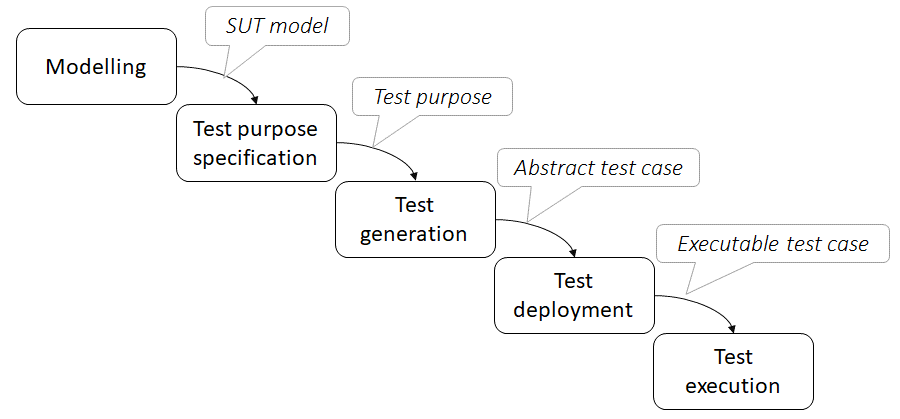
\includegraphics[width=\textwidth]{images/presentation/MBTWorkflow.png}
%            \caption{Potential MBT workflow.}
%            \label{fig:mbt_workflow}
%        \end{figure}
%    \end{frame}

    \begin{frame}
        \frametitlecont{}
        \begin{definitionboxnopause}[Test Generation]
            Derivation of abstract test sequences from the state space of a SUT model using test purposes as guiding constraints.
        \end{definitionboxnopause}
        \pause
        \bigskip
        \par Requirements for automation:
        \pause
        \begin{itemize}[<+->]
            \item notation for expressing test purposes;
            \item machine-interpretable modelling formalism.
        \end{itemize}
        \pauseafteritemize
        \bigskip
        \par Benefits of automation:
        \pause
        \begin{itemize}[<+->]
            \item eliminate redundant activities;
            \item prevent human errors;
            \item reduce costs.
        \end{itemize}
    \end{frame}
% END SUBSECTION: MBT

% BEG SUBSECTION: UPPAAL
    \subsection{UPPAAL}
    \begin{frame}
        \frametitlestore{Context -- UPPAAL}
        \begin{definitionboxnopause}[UPPAAL Timed Automata (UTA)]
            Modeling formalism where systems are represented as networks of state transition graphs annotated with timing constraints.
        \end{definitionboxnopause}
        \pause
        \bigskip
        \par Facilitates modeling of real-time systems.
        \pause
        \bigskip
        \par The UPPAAL toolkit includes the following core tools:
        \pause
        \begin{itemize}[<+->]
            \item graphical environment for defining UTA models,
            \item simulator which allows user to execute a model and observe its behavior,
            \item model-checker (\monofont{verifyta}) -- provides tools for the formal verification of correctness properties for the model (and the generation of \textit{witness traces} which prove these properties).
        \end{itemize}
    \end{frame}

    \begin{frame}
        \frametitlecont{}
        \begin{figure}
            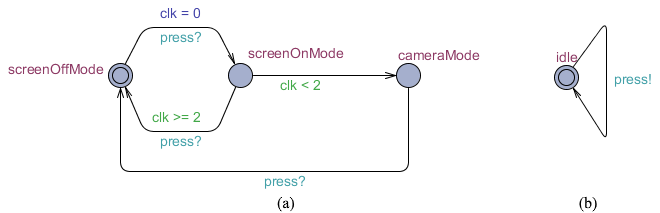
\includegraphics[width=0.8\textwidth]{images/presentation/ExampleUPPAALAutomata.png}
            \caption{Example UPPAAL automata: (a) smartphone, (b) user.}
            \label{fig:uppaal_example}
        \end{figure}
    \end{frame}

    \begin{frame}
        \frametitlecont{}
        \par UPPAAL's property specification language can be used to express test purposes.
        \pause
        \begin{columns}[t] % T - for top alignment.
            \column{0.48\textwidth}
                \par Formula types:
                \pause
                \begin{itemize}[<+->]
                    \item state formulae: \monofont{systemProcess.workCompleted};
                    \item path formulae: \monofont{E<>systemProcess.workCompleted}.
                \end{itemize}
                %\pauseafteritemize
            \column{0.48\textwidth}
                \begin{figure}
                    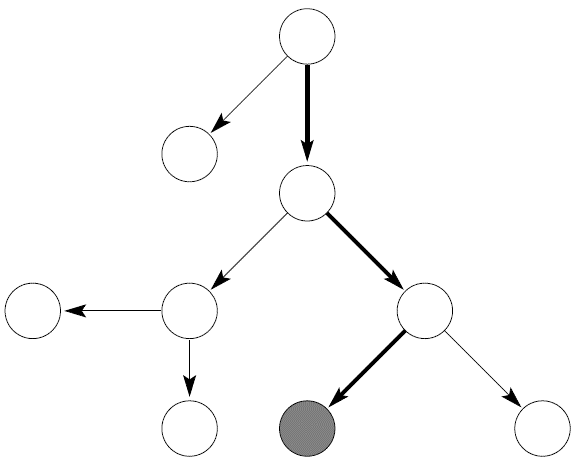
\includegraphics[width=0.75\textwidth]{images/presentation/ExamplePropertyVerificationSearch.png}
                    \caption{Verification of reachability property \texttt{E<>p}.}
                    \label{fig:verifyta_reachability}
                \end{figure}
        \end{columns}
    \end{frame}
% END SUBSECTION: UPPAAL

% BEG SUBSECTION: TDL
    \subsection{Test Purpose Specification Language \TDLTP{}}
    \begin{frame}
        \frametitlestorepause{Context -- Test Purpose Specification Language \TDLTP{}}
        \par Limitations of UPPAAL test purpose specification language:
        \pause
        \begin{itemize}[<+->]
            \item temporal operators cannot be nested;
            \item complex test purposes require manual modification of SUT model;
            \item UPPAAL MBT only feasible for expert users.
        \end{itemize}
        \pauseafteritemize
        \bigskip
        \par Solution: \vskip1ex
        %\pause
        \begin{textbox}
            Evelin Halling, Jüri Vain, Artem Boyarchuk, and Oleg Illiashenko,\\
            \textbf{"Test Scenario Specification Language for Model-based Testing"},\\
            \textit{International Journal of Computing}, 2019.
        \end{textbox}
    \end{frame}

    \begin{frame}
        \frametitlestorecont{Context -- Test Purpose Spec. Language \TDLTP{}}
        \par In \TDLTP{}:
        \pause
        \begin{itemize}[<+->]
            \item test purposes are encoded as logical expressions, e.g.\\
                \monofont{A(TS1) \vertmidtilde> E(TS2) \& E(TS3)};
            \item ground level terms in the expression are references to sets of transitions in the SUT model;
            \item once expression is interpreted, a behaviorally equivalent test model is produced;
            \item test model is an extension of SUT model which contains a \textit{property recognizer automata} tree that structurally mirrors the abstract syntax tree (AST) of the expression;
            \item root automaton in the recognizer tree (\monofont{stopwatch}) is intended to be used in the UPPAAL reachability query \monofont{E<>stopwatch.pass};
            \item witness trace generated per query is an abstract test case.
        \end{itemize}
    \end{frame}

    \begin{frame}
        \frametitlecont{}
        \begin{figure}
            \centering
            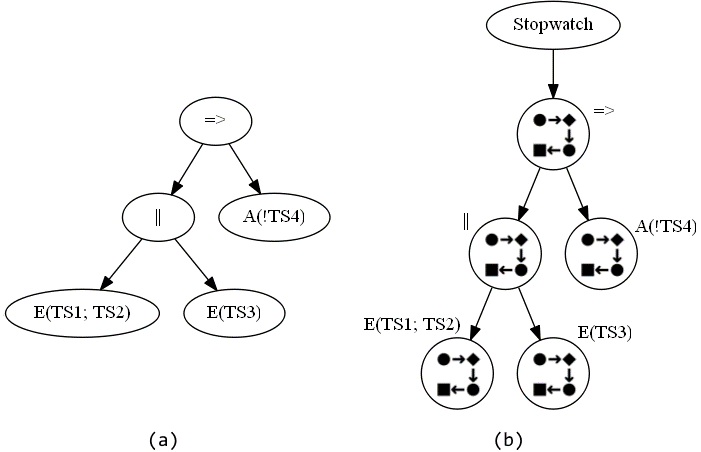
\includegraphics[width=0.75\textwidth]{images/presentation/ASTVsRecognizerTree.png}
            \caption{Comparison of \TDLTP{} AST (a) and corresponding recognizer tree (b).}
            \label{fig:tdl_ast_vs_recognizer_tree}
        \end{figure}
    \end{frame}

    \begin{frame}
        \frametitlecont{}
        \begin{figure}
            \centering
            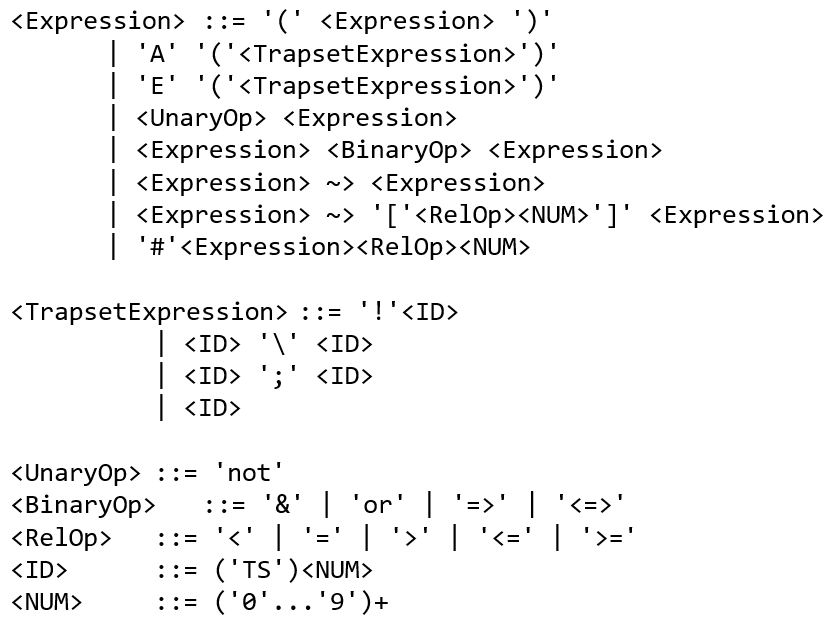
\includegraphics[width=0.65\textwidth]{images/presentation/TdlExpressionSyntax.png}
            \caption{\TDLTP{} grammar.}
            \label{fig:tdl_grammar}
        \end{figure}
    \end{frame}

% TODO: Slide relating model to expression; recognizer tree.
% END SUBSECTION: TDL
%---------------------
% BEG SECTION: CONTEXT

% BEG SECTION: OBJECTIVE
%-----------------------
    \section{Objective}
    \begin{frame}
        \frametitlestore{Objective}
        \begin{block}{Goal Statement}
            Implement an interpreter that accepts as input:
            %\pause
            \begin{itemize}%[<+->]
                \item a \TDLTP{} expression,
                \item a UPPAAL SUT model,
            \end{itemize}
            %\pauseafteritemize
            and produces a \textbf{test model} as output.
        \end{block}
        \pause
        \bigskip
        \par \textit{Caveats}:
        \pause
        \begin{itemize}[<+->]
            \item efficiency is not an immediate concern;
            \item assume model validity wrt system requirements.
        \end{itemize}
    \end{frame}

    \begin{frame}
        \frametitlecont{}
        \begin{figure}
            %\centering
            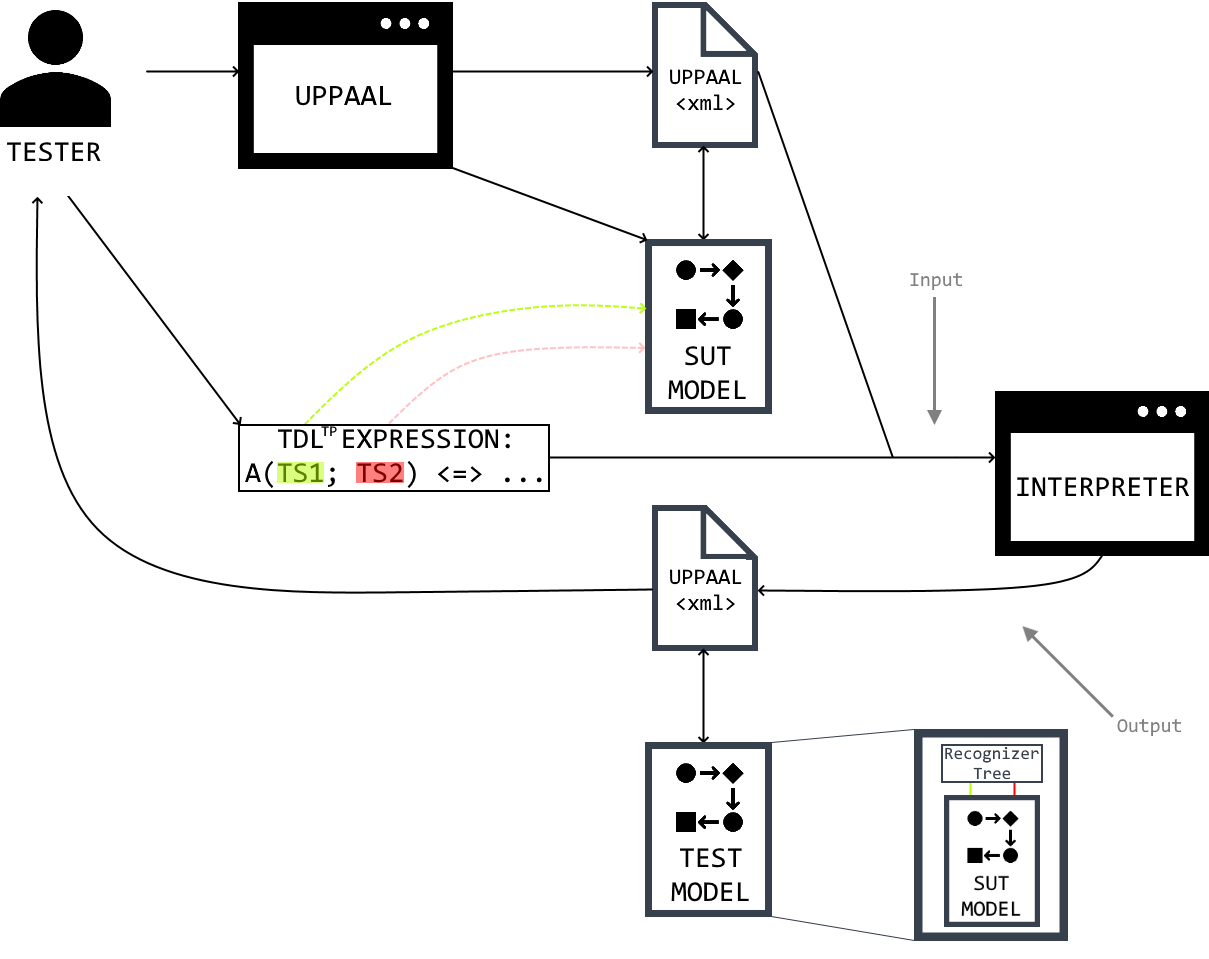
\includegraphics[width=0.76\textwidth]{images/presentation/InteractionDiagram.png}
            \caption{Interaction diagram.}
            \label{fig:interaction}
        \end{figure}
    \end{frame}
%-----------------------
% END SECTION: OBJECTIVE

% BEG SECTION: IMPLEMENTATION
%----------------------------
\section{Implementation}
% BEG SUBSECTION: APPROACH
    \subsection{Approach}
    \begin{frame}
        \frametitlestore{Implementation -- Approach}
        \par Takes inspiration from Component-Based Development (CBD).
        \pause
        \bigskip
        \par General process:
        %\pause
        \begin{itemize}[<+->]
            \item identify necessary sub-functionalities;
            \item design initial component layout;
            \item implement bottom-up;
            \item adjust when appropriate.
        \end{itemize}
        \pauseafteritemize
        \bigskip
        \par Benefits:
        \pause
        \begin{itemize}[<+->]
            \item limit coupling;
            \item enforce reusability;
            \item facilitate refactoring.
        \end{itemize}
    \end{frame}
% END SUBSECTION: APPROACH

% BEG SUBSECTION: STRUCTURE
    \subsection{Structure}
    \begin{frame}
        \frametitlestore{Implementation -- Structure}
        \begin{figure}
            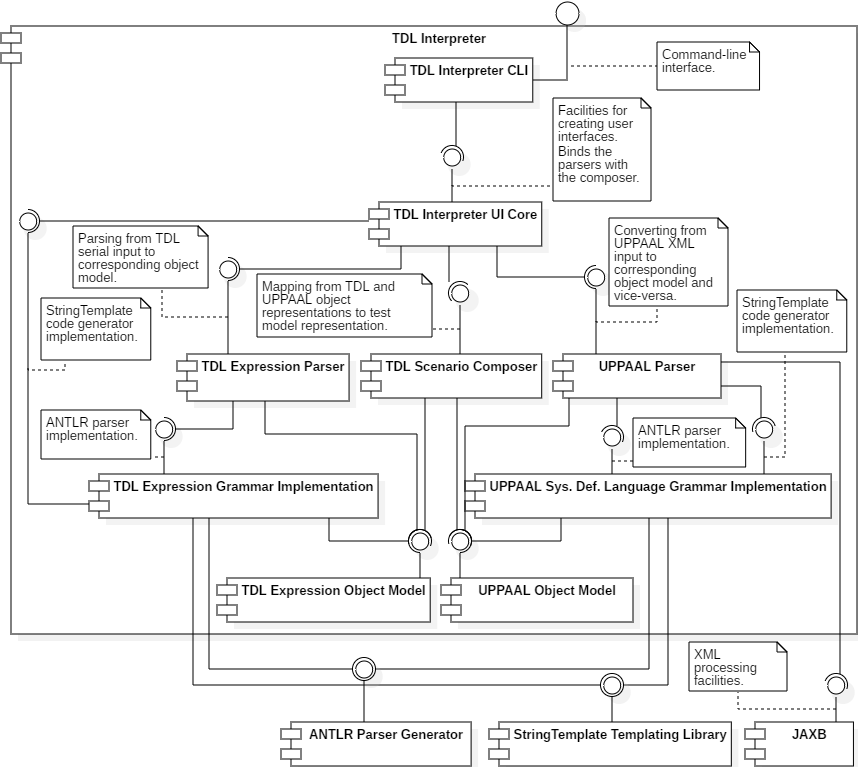
\includegraphics[height=0.8\textheight]{images/presentation/ComponentDiagram.png}
            \caption{Partial component diagram.}
            \label{fig:components}
        \end{figure}
    \end{frame}
% END SUBSECTION: STRUCTURE

% BEG SUBSECTION: DEMONSTRATION
    \subsection{Demonstration}
    \begin{frame}
        \frametitlestorepause{Demonstration}
        \begin{figure}
            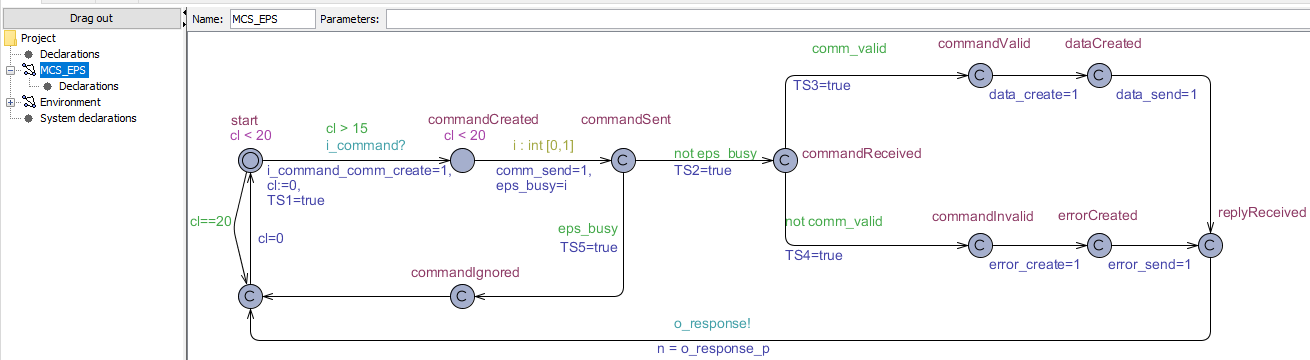
\includegraphics[width=\textwidth]{images/presentation/InputModel.png}
            \caption{Example UPPAAL input model.}
            \label{fig:example_input_model}
        \end{figure}
        \pause
        \begin{figure}
            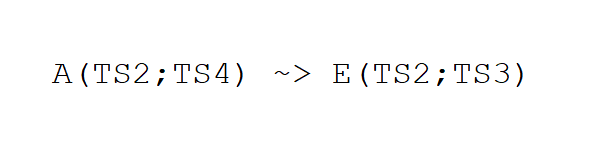
\includegraphics[width=0.5\textwidth]{images/presentation/InputExpression.png}
            \caption{Example \TDLTP{} input expression.}
            \label{fig:example_input_expression}
        \end{figure}
    \end{frame}

    \begin{frame}
        \frametitlecont{}
        \begin{figure}
            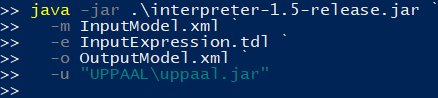
\includegraphics[width=0.6\textwidth]{images/presentation/CallExample.png}
            \caption{Call to interpreter command-line interface.}
            \label{fig:example_call}
        \end{figure}
    \end{frame}

    \begin{frame}
        \frametitlecont{}
        \begin{figure}
            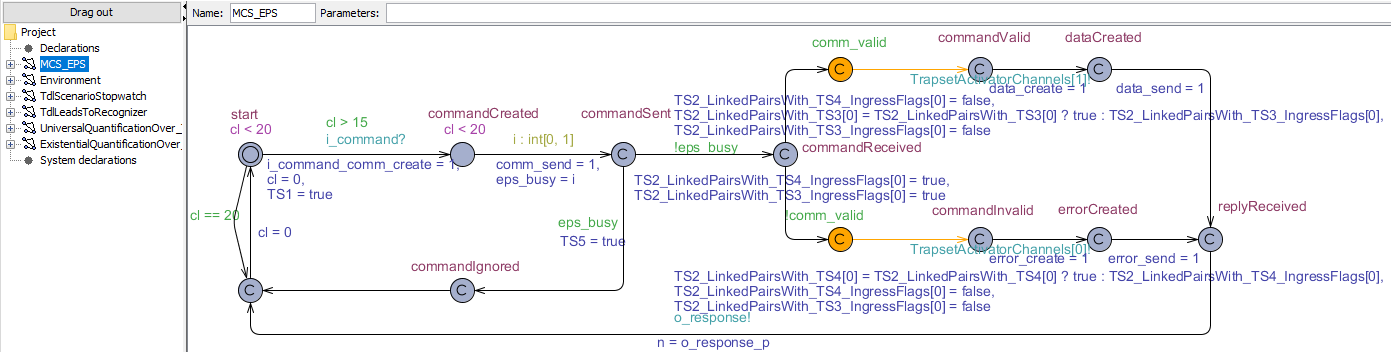
\includegraphics[width=\textwidth]{images/presentation/OutputModel.png}
            \caption{Example test model.}
            \label{fig:example_test_model}
        \end{figure}
    \end{frame}
% END SUBSECTION: DEMONSTRATION
%----------------------------
% BEG SECTION: IMPLEMENTATION

% BEG SECTION: VALIDATION
%------------------------
    \section{Validation}
    \begin{frame}
        \frametitlestore{Validation}
        \par Observations:
        \pause
        \begin{itemize}[<+->]
            \item Multiple component interactions are involved in test model generation -- need to ensure the output conforms to rules of \TDLTP{}.
            \item Rules are well-defined, so automated validation is feasible (but complicated).
            \item Due to time limitations, most validation efforts were manual.
            \item User input processing partially covered by automated tests.
        \end{itemize}
    \end{frame}

    \begin{frame}
        \frametitlecont{}
        \par Automated tests for language parsers:
        \pause
        \begin{itemize}[<+->]
            \item \textit{Strategy}: structural validation of abstract syntax tree (AST).
            \item \textit{Approach}: s-expressions (notation for representing tree structures) as common intermediate format.
            \item 109 automated test cases -- handful of programming defects discovered and resolved.
        \end{itemize}
        \pauseafteritemize
        \begin{figure}
            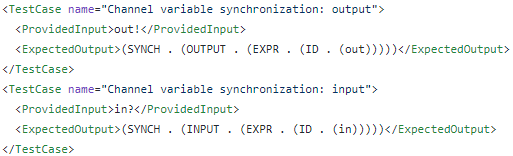
\includegraphics[width=0.75\textwidth]{images/presentation/AutomatedParserTestCase.png}
            \caption{Example automated UPPAAL language parser test cases.}
            \label{fig:uta_parser_test_case}
        \end{figure}
    \end{frame}

    \begin{frame}
        \frametitlecont{}
        \par Manual integration tests:
        %\pause
        \begin{itemize}[<+->]
            \item \textit{Strategy}: define basic input model, \TDLTP{} expression.
            \item \textit{Approach}: apply expression to model using interpreter, validate visually.
            \item 95 manual test cases -- 4 logical errors, 1 user-friendliness issue, handful of code defects discovered and resolved.
        \end{itemize}
        \pauseafteritemize
        \begin{figure}
            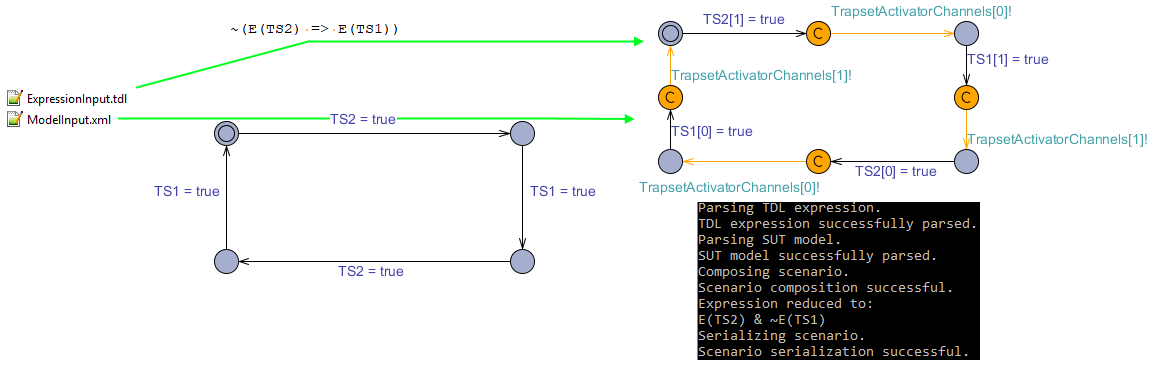
\includegraphics[width=\textwidth]{images/presentation/ManualTestCase.png}
            \caption{Example integration test case.}
            \label{fig:integration_test_case}
        \end{figure}
    \end{frame}
%------------------------
% BEG SECTION: VALIDATION

% BEG SECTION: SUMMARY & FUTURE WORK
%-----------------------------------
    \section{Summary}
    \begin{frame}
        \frametitlestore{Summary}
        \par In summary:
        \pause
        \begin{itemize}[<+->]
            \item \textit{Goal}: implement an interpreter based on the theory of \TDLTP{}.
            \item \textit{Assessment}: successfully implemented, sufficiently validated.
            \item The interpreter will find use in a prototype environment for MBT of cyber-physical systems under development at TalTech for several years;
            \item Project management/code repository: \href{https://gitlab.cs.ttu.ee/Tanel.Prikk/iapb/boards}{TalTech GitLab}.
        \end{itemize}
        \pauseafteritemize
        \bigskip
        \par Future work:
        \pause
        \begin{itemize}[<+->]
            \item resolve major open questions in \TDLTP{} theory uncovered as part of this work (discussed in Sections 5.3, 5.2.2, Appendices 5 -- 6 of the thesis);
            \item expand automated test coverage;
            \item graphical user interface for annotating input model according to the \TDLTP{} input expression;
            \item codebase: apply generalizations where applicable.
        \end{itemize}
    \end{frame}

    \begin{frame}
        \frametitlecont{}
        \par \href{https://toggl.com/app/bookmark/03a8815eedda53a54dcc49829427f8dc}{\textit{toggl}} was used to record time spent on the thesis.
        \begin{figure}
            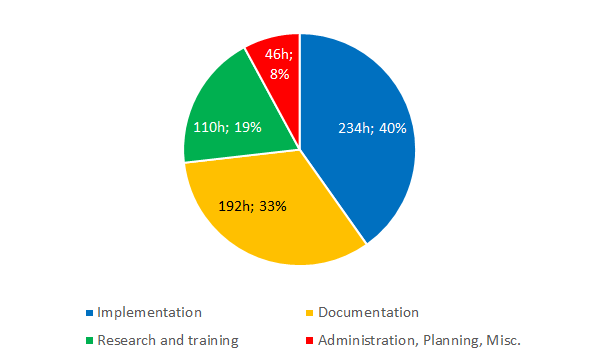
\includegraphics[width=0.75\textwidth]{images/presentation/TimeSplit.png}
            \caption{Overview of thesis scope.}
            \label{fig:time_split}
        \end{figure}
    \end{frame}
%-----------------------------------
% BEG SECTION: SUMMARY & FUTURE WORK
%===================================
% END CONTENT FRAMES

% BEG FINAL FRAME
    \begingroup
        \setbeamercolor{background canvas}{bg=TalTechGray} % Gray background.
        \setbeamertemplate{navigation symbols}{} % No nav symbols.
        \begin{frame}[plain, noframenumbering]{}
        \end{frame}
    \endgroup
% END FINAL FRAME
\end{document}
